% beamer


\documentclass[aspectratio=169]{beamer}
\usetheme{Madrid}
\usecolortheme{default}

% Packages
\usepackage{graphicx}
\usepackage{amsmath}
\usepackage{amssymb}
\usepackage{booktabs}
\usepackage{listings}
\usepackage{xcolor}
\usepackage{hyperref}
\usepackage{tikz}
\usepackage{xfp}
\usepackage{subcaption}
% duplicate graphicx removed
\usepackage{pgffor} % [EN] Required for \foreach loop / [CN] 用于foreach循环
\usetikzlibrary{shapes,arrows,positioning}

% Code listing settings
\lstset{
  basicstyle=\ttfamily\footnotesize,
  breaklines=true,
  frame=single,
  numbers=left,
  numberstyle=\tiny\color{gray},
}
\title{QMDraw Data Analysis}
\author{Tian Baiting}
\institute{SAMURAI Collaboration}

% Footer customization
\setbeamertemplate{footline}[frame number]

% 在导言区加入这段代码
\AtBeginSection[]
{
  \begin{frame}
    \frametitle{Outline}
    \tableofcontents[currentsection, hideothersubsections]
  \end{frame}
}

\begin{document}

% Title slide
\begin{frame}
\titlepage
\end{frame}

\begin{frame}
  %  list of content 生成目录
\tableofcontents  
\end{frame}
% \section{config}

\section{input}

\begin{frame}{Input Momentum Analysis (QMD Model)}
    \begin{itemize}
        \item \textbf{Objective}: Analyze the momentum distribution of breakup products to guide detector configuration.
        \item \textbf{Data Source}: QMD simulation data for $^{208}$Pb target.(qmd ypol has Pb208 Xe130, zpol has Sn112 Sn124 Xe130)
        \item \textbf{Methodology}:
        \begin{itemize}
            \item Analyzed Proton and Neutron momentum in Y-polarization and Z-polarization modes.
            \item Used Python/ROOT notebook (\texttt{zpol\_ypol\_show\_approx\_P.ipynb}) for visualization.
            \item Focused on $P_z$ vs $P_\perp$ distributions.
        \end{itemize}
    \end{itemize}
\end{frame}

\begin{frame}{Momentum Statistics \& Reference Selection}
    \begin{columns}
        \column{0.5\textwidth}
        $P = \sqrt{(E)^2 - (m)^2} = \sqrt{(190+938)^2 - (938)^2} MeV/c = 625.5MeV/c$
        \textbf{Observed Statistics (from Log)}
        \begin{itemize}
            \item \textbf{Proton $P_z$}: Mean $\approx 600$ MeV/c (Y-pol), $\approx 635$ MeV/c (Z-pol).
            \item \textbf{Neutron $P_z$}: Mean $\approx 612$ MeV/c.
            \item \textbf{$P_\perp$}: Typically $50 - 90$ MeV/c.
        \end{itemize}
        
        \column{0.5\textwidth}
        \begin{alertblock}{Reference Kinematics}
            To optimize the detector coverage, we select the following reference momentum for protons:
            \begin{itemize}
                \item \textbf{$P_z = 627$ MeV/c}
                \item \textbf{$P_x = \pm 100 , \pm 150$ MeV/c }
            \end{itemize}
        \end{alertblock}
    \end{columns}
\end{frame}


\begin{frame}{Proton Momentum Distributions}
    \begin{columns}
        \column{0.5\textwidth}
        \centering
        \textbf{Y-Polarization}\\
        \includegraphics[width=0.9\textwidth]{../../note_log/assets/log202511/image.png}
        \column{0.5\textwidth}
        \centering
        \textbf{Z-Polarization}\\
        \includegraphics[width=0.9\textwidth]{../../note_log/assets/log202511/image-2.png}
    \end{columns}
    \vspace{0.2cm}
    \centering
    \small{Proton $P_z$ vs $P_\perp$ distributions showing the region of interest around $P_z \approx 600$ MeV/c.}
\end{frame}

\begin{frame}{Neutron Momentum Distributions}
    \begin{columns}
        \column{0.5\textwidth}
        \centering
        \textbf{Y-Polarization}\\
        \includegraphics[width=0.9\textwidth]{../../note_log/assets/log202511/image-1.png}
        \column{0.5\textwidth}
        \centering
        \textbf{Z-Polarization}\\
        \includegraphics[width=0.9\textwidth]{../../note_log/assets/log202511/image-3.png}
    \end{columns}
    \vspace{0.2cm}
    \centering
    \small{Neutron distributions show similar $P_z$ trends.}
\end{frame}

\section{correlation between p and n}



\section{cut on unphysical breakup}





\section{obersevation R }


\begin{frame}{Our Probe: The Isovector Reorientation (IVR) Effect}
    \begin{columns}[T]
        \begin{column}{0.6\textwidth}
        \centering
    \includegraphics[width=\columnwidth]{./img/isovector_reorientaton.png}
    \end{column}
    \begin{column}{0.4\textwidth}
    \tiny{
    \begin{align*}
        E_{\text{sym}}(\rho) = \frac{C_{s,k}}{2} \left(\frac{\rho}{\rho_0}\right)^{2/3} + \\ \frac{C_{s,p}}{2} \left(\frac{\rho}{\rho_0}\right)^{\gamma}
    \end{align*}
    }


    $$
    \small
    \gamma \uparrow \Rightarrow \frac{dE_{\text{sym}}}{d\rho} \downarrow \Rightarrow F_v \downarrow
    $$
    \end{column}
\end{columns}

    \begin{itemize}
        \item[\textcolor{blue}{$\blacklozenge$}] In peripheral scattering of a polarized deuteron, the \textbf{isovector nuclear force} acts as a torque.
        \begin{itemize}
            \item Attractive for protons
            \item Repulsive for neutrons
        \end{itemize}
        \item[\textcolor{blue}{$\blacklozenge$}] This causes an "extra rotation" of the deuteron before it breaks up.
        \item[\textcolor{blue}{$\blacklozenge$}] This makes it a \textbf{clean probe}: sensitive to the isovector potential (\(E_{\text{sym}}\)) but insensitive to the isoscalar potential.
    \end{itemize}


    %  这里加入 Px+Px意义, Px-Px.
\end{frame}


\begingroup
    \setbeamertemplate{background}{%
        \begin{tikzpicture}[remember picture, overlay]
            \node[at=(current page.east), anchor=east, xshift=0cm, opacity=0.3] {
                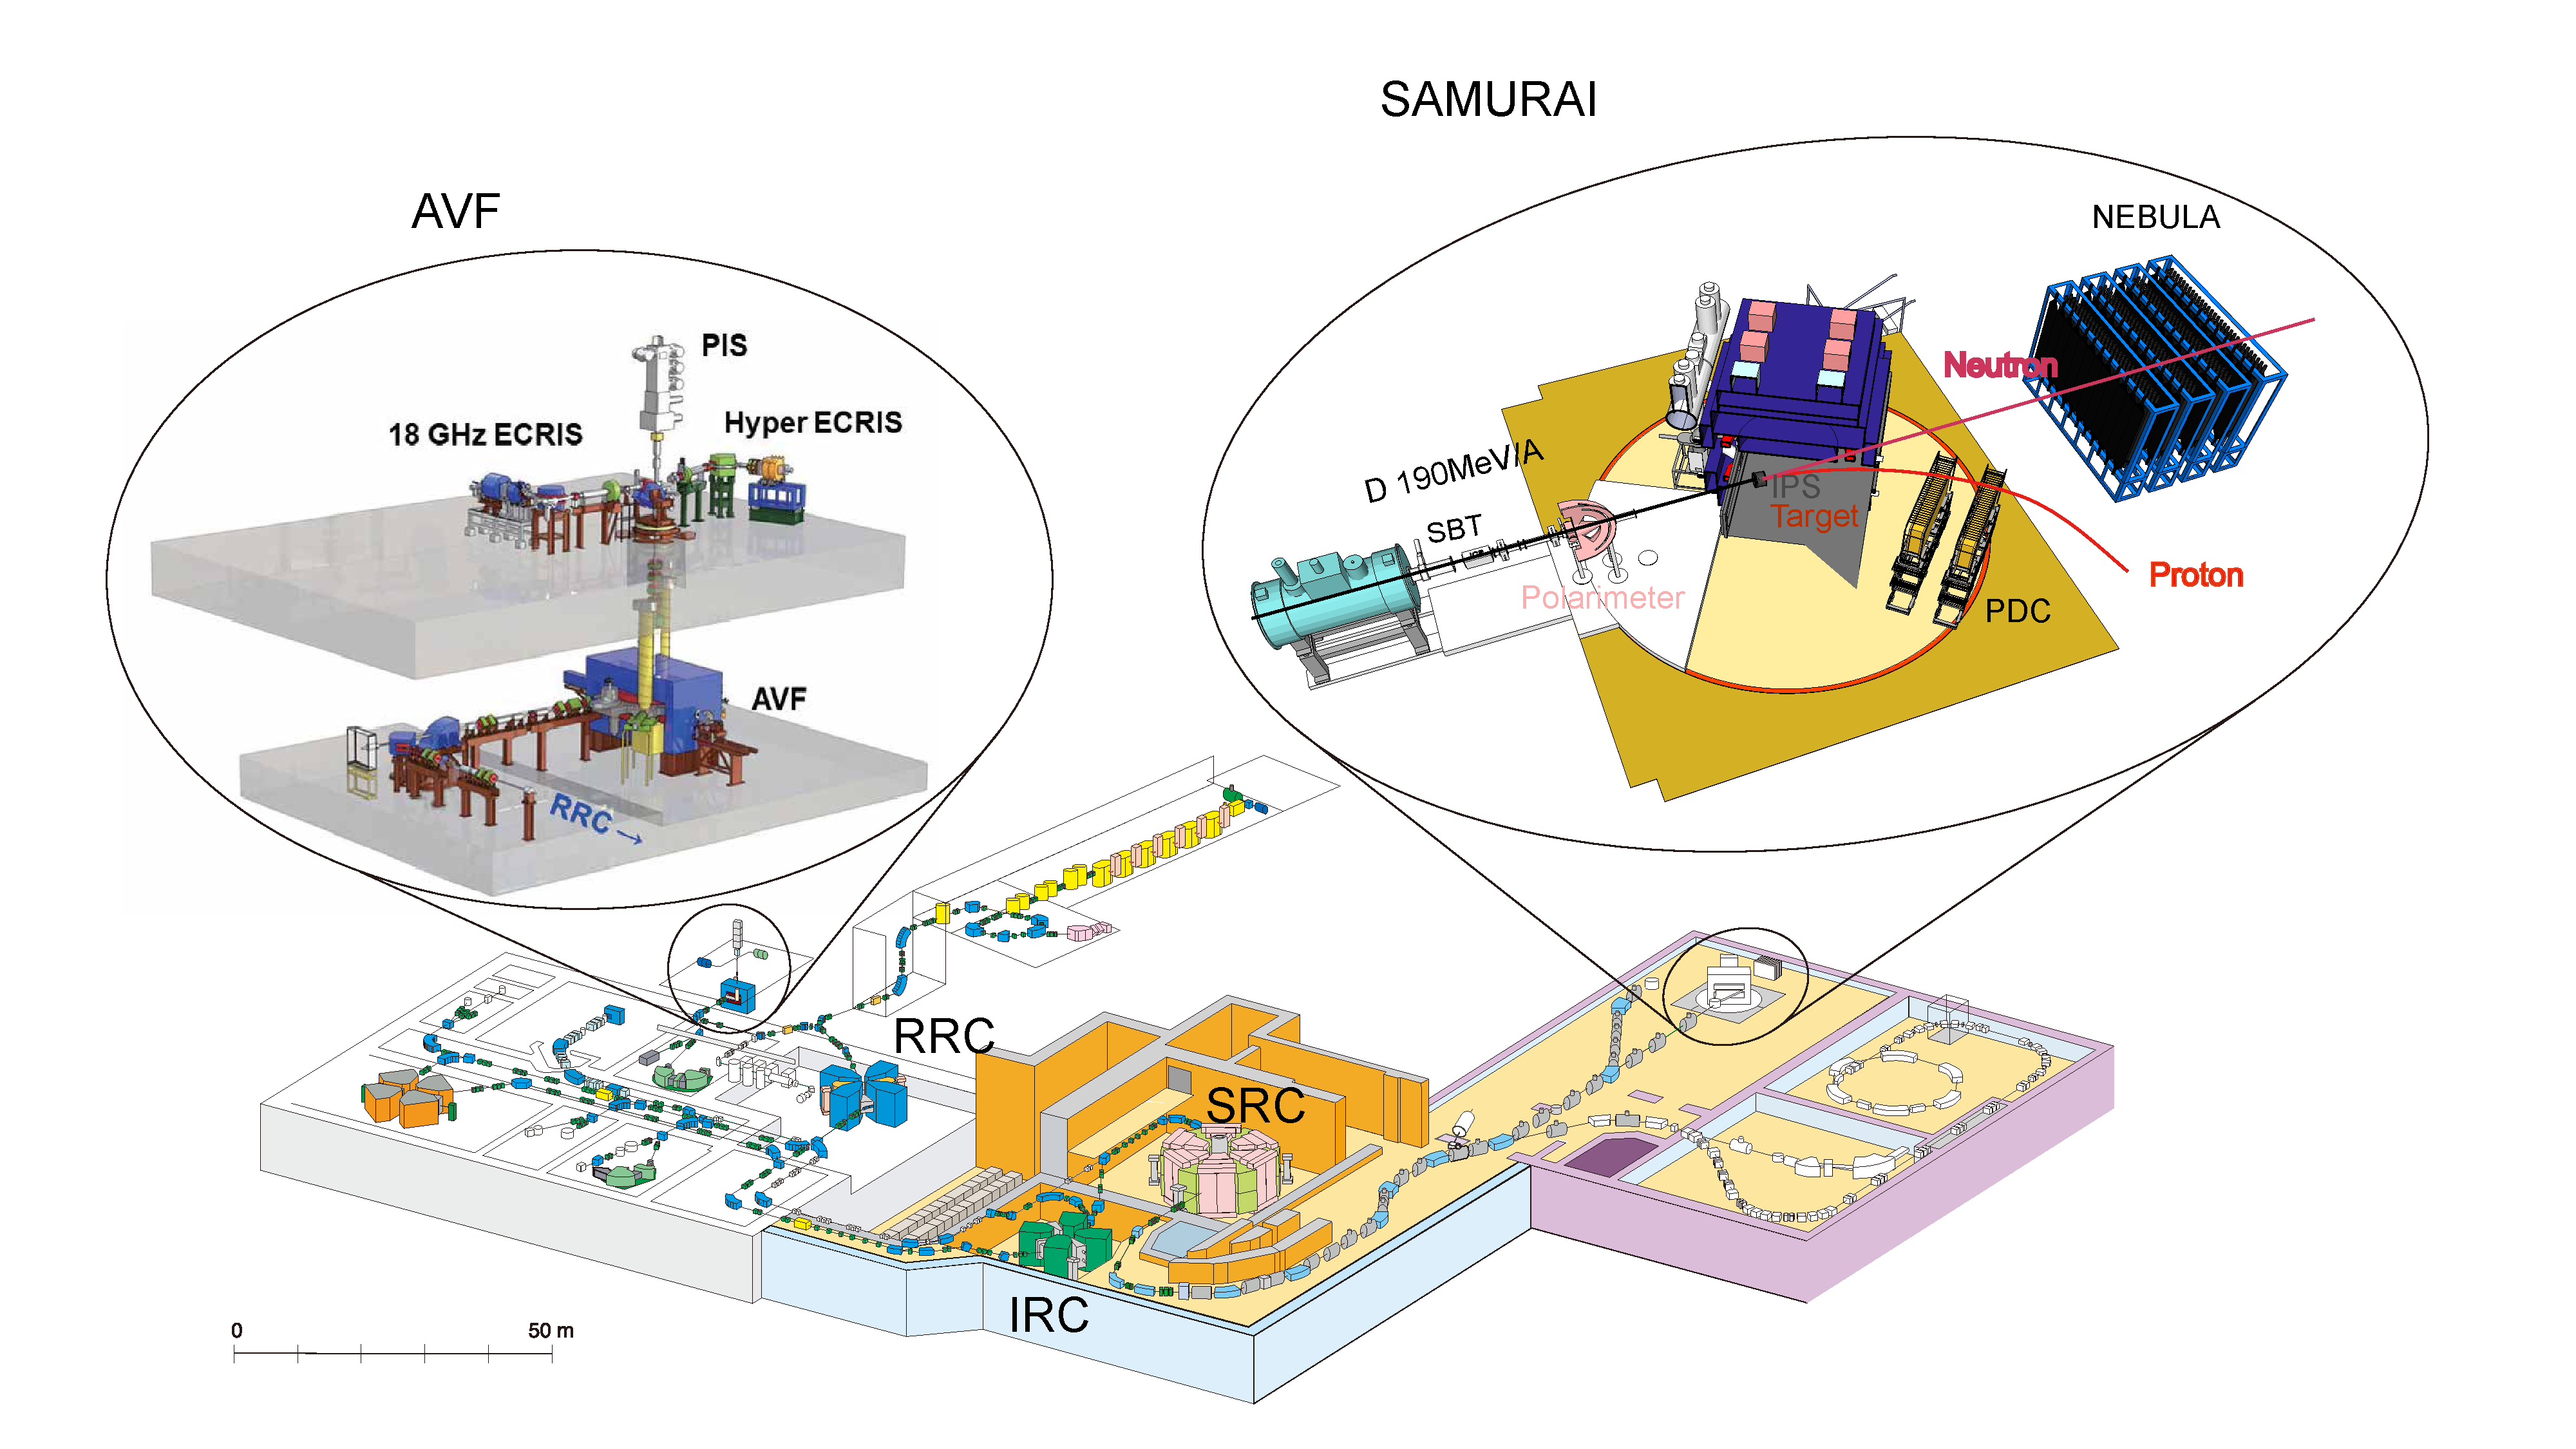
\includegraphics[height=0.6\paperheight]{img/schematic_of_beamline.pdf}
            };
        \end{tikzpicture}
    }
    \begin{frame}{Outline}
        \tableofcontents[currentsection]
    \end{frame}
\endgroup
% 恢复默认背景,防止影响后续页面
\setbeamertemplate{background}{}

\begin{frame}{The Signature: Asymmetry in Breakup Momenta}
    \begin{columns}[T]
        \begin{column}{0.5\textwidth}
            \vfill
            % 图片占位符: Diagram defining px_p and px_n
            \includegraphics[width=\columnwidth]{./img/pol.pdf}
                     \vfill
            % 图片占位符: Plot from Prof. Xiao's talk (Slide 9) showing asymmetric vs symmetric distribution
            \includegraphics[width=\columnwidth]{./img/unpol.pdf}
        \end{column}
        \begin{column}{0.5\textwidth}
     X: total $P_x$,measures the impact parameter b
approximately.

$\gamma \uparrow  \quad \rightarrow \quad P^p_x - P^n_x \downarrow$


     \begin{itemize}
        \item For a \textbf{polarized} beam, the distribution is asymmetric. 
        \item For an \textbf{unpolarized} beam, the distribution is symmetric.
        \item The degree of asymmetry is our signal!
    \end{itemize}
        \end{column}
    \end{columns}

\end{frame}



\section{obersevation R cut on $P_{\perp}$}

\begin{frame}
    $P_{\perp}$ reflects the impact parameter $b$ of the collision as we mentioned before.

    Here we concentrate on which range of $P_{\perp}$ has more significant IVR effect. Thus we can foucus on that range in the reconstruction proton and neutron momenta.
\end{frame}



\section*{backup}


\end{document}